\documentclass{standalone}

\usepackage{circuitikz}

\begin{document}

% INT_AY21_L20_Fig05_Vel_in_central_force.png

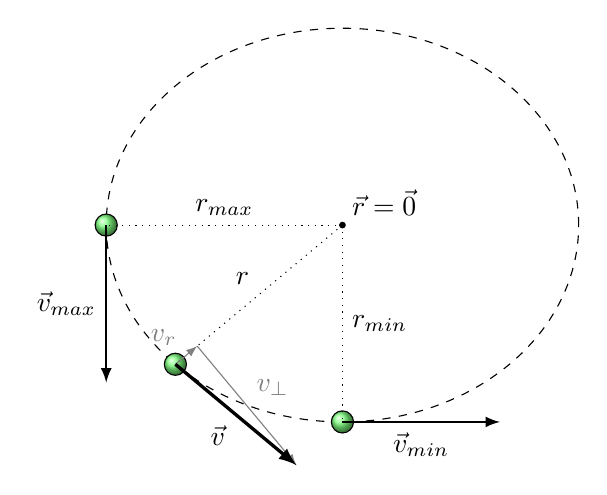
\begin{tikzpicture}[> = latex]

	% Definitions
	
	\def\v{2}		% Velocity vector size
	\def\a{3}		% Semi-major axis
	\def\b{2.5}		% Semi-minor axis
	\def\Q{225}		% Angular location of intermediate position
	
	% Velocity component along radial vector
	
	\pgfmathparse{-(\a^2 - \b^2) * sin(\Q) * cos(\Q) / (\a^2 * cos(\Q) ^2 + \b^2 * sin(\Q)^2)}
	\let\vPar\pgfmathresult
	
	% Velocity component perpendicular to radial vector
	
	\pgfmathparse{-\a * \b / (\a^2 * cos(\Q) ^2 + \b^2 * sin(\Q)^2)}
	\let\vPerp\pgfmathresult
	
	% Magnitude of unscaled vector
	
	\pgfmathparse{1 / sqrt(\a^2 * sin(\Q) ^2 + \b^2 * cos(\Q)^2)}
	\let\mag\pgfmathresult

	% Orbit
	
	\draw [dashed] (0, 0) circle [x radius = \a, y radius = \b];
	
	% Central point
	
	\draw [fill = black] (0, 0) circle (1 pt) node [above right] {${\vec r} = {\vec 0}$};
	
	% Object at largest radius
	
	\draw [ball color = green!50] (-\a, 0) circle (4 pt);
	\draw [dotted] (0, 0) -- node [above] {$r_{max}$} (-\a, 0);
	\draw [->, thick] (-\a, 0) -- node [left] {${\vec v}_{max}$} (-\a, -\v);
	
	% Object at intermediate radius (total kluge from previous code)
	
	\draw [ball color = green!50] ({\a * cos(\Q)}, {\b * sin(\Q)}) circle (4 pt);
	\draw [dotted] (0, 0) -- node [above left] {$r$} ({\a * cos(\Q)}, {\b * sin(\Q)});
	
	\draw [->, gray] ({\a * cos(\Q)}, {\b * sin(\Q)}) -- node [midway, above left] {$v_r$} ++ ({\v * \mag * \vPar * \a * cos(\Q)}, {\v * \mag * \vPar * \b * sin(\Q)}) coordinate (end-vr);
	\draw [->, gray] (end-vr) -- node [midway, above right] {$v_\perp$} ++ ({\v * \mag * \vPerp * \b * sin(\Q)}, {-\v * \mag * \vPerp * \a * cos(\Q)});
	\draw [very thick, ->] ({\a * cos(\Q)}, {\b * sin(\Q)}) -- node [below left] {${\vec v}$} ++ ({-\v * \mag * \a * sin(\Q)}, {\v * \mag * \b * cos(\Q)});
	
	% Object at smallest radius
	
	\draw [ball color = green!50] (0, -\b) circle (4 pt);
	\draw [dotted] (0, 0) -- node [right] {$r_{min}$} (0, -\b);
	\draw [->, thick] (0, -\b) -- node [below] {${\vec v}_{min}$} (\v, -\b);

\end{tikzpicture}

\end{document}